\label{sec:dthreadsevaluation}

We perform our evaluation on an Intel Core 2 dual-processor CPU system, equipping with 16GB of RAM. Each processor is a 4-core 64-bit Xeon, running at 2.33GHZ with a 4MB L2 cache. The operating system is an unmodified CentOS 5.5, running with Linux kernel version 2.6.18-194.17.1.el5.

\subsection{Methodology}

We evaluate the performance and scalability of \dthreads{} (versus CoreDet and \pthreads{}) across the PARSEC~\cite{parsec} and Phoenix~\cite{phoenix-hpca} benchmark suites.  

In order to compare performance directly against CoreDet, which relies on the LLVM infrastructure, all benchmarks are compiled with the LLVM compiler at the ``-O3'' optimization level~\cite{LLVM:CGO04}. Since \dthreads{} does not currently support 64-bit binaries, all benchmarks are compiled for 32 bit environments (using the ``-m32'' compiler flag). Each benchmark is executed ten times on a quiescent machine. To reduce the effect of outliers, results with the worst and best performance for each benchmark are discarded,
so each result is the average of the remaining eight runs.

\textbf{Tuning CoreDet:} 
The performance of CoreDet~\cite{Bergan:2010:CCR:1736020.1736029} is extremely sensitive to three parameters: the granularity for the ownership table (in bytes), the quantum size (in number of instructions retired), and the choice between full serial mode and reduced serial mode. We compare the performance and scalability of \dthreads{} with the best possible results that we could obtain for CoreDet on our system---that is, with the lowest average normalized
runtime---after an extensive search of the parameter space (six possible granularities and 8 possible quanta, for each benchmark). The results presented here are for a 64-byte granularity, a quantum size of 100,000 instructions, and in full serial mode.

\textbf{Unsupported Benchmarks}: We do not include results for 7 benchmarks from PARSEC, since they do not currently work with \dthreads{} (note that many of these also do not work for CoreDet). \texttt{vips} and \texttt{raytrace} would not build as 32-bit executables; \texttt{bodytrack}, \texttt{facesim}, and \texttt{x264} depend on sharing of stack variables;
\texttt{fluidanimate} uses ad-hoc synchronization, so it cannot run without modifications; and \texttt{freqmine} does not use \pthreads{}.

 
\textbf{Scalability Experiment}: For all scalability experiments, we logically disable CPUs using Linux's CPU hotplug mechanism, which allows us to disable or enable a specific CPU by writing ``0'' or ``1'' to a file: \texttt{/sys/devices/system/cpu/cpuN/online}.

\subsection{Determinism}

We first experimentally verify \dthreads{}' ability to ensure determinism by executing the \emph{racey} determinism tester~\cite{1508256}. This stress test contains, as its name suggests, numerous data races and is thus extremely sensitive to memory-level non-determinism. \dthreads{} reports the same results for 2,000 runs. We also verify that the schedules and outputs of all benchmarks of every execution are identical.

\subsection{Performance}
\label{sec:performance}

\begin{figure*}[!t]
{\centering
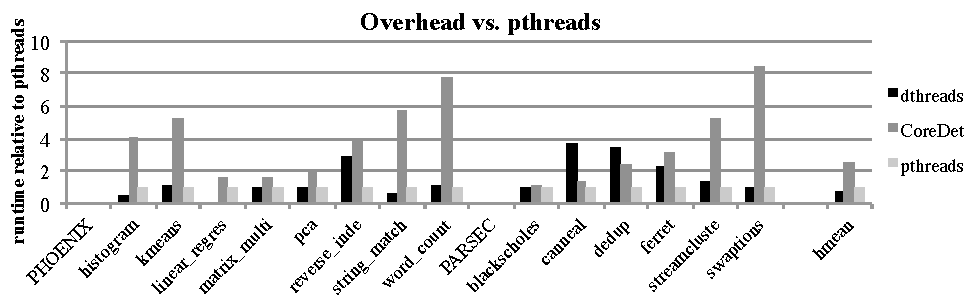
\includegraphics[width=6in]{dthreads/figure/overhead-figure}
\caption{Normalized execution time with respect to \pthreads{} and CoreDet(lower is better). For 9 of the 14 benchmarks, \dthreads{} runs nearly as fast or faster than \pthreads{}, while providing deterministic behavior.\label{fig:performance}}
}
\end{figure*}

\begin{table*}[!t]
\centering
\resizebox{\columnwidth}{!}{
\begin{tabular}{l|rr|l}
{\bf \small Benchmark} & $\frac{\mbox{\bf \small CoreDet}}{\mbox{\bf \small \pthreads{}}}$ & $\frac{\mbox{\small \bf \dthreads{}}}{\mbox{\small \bf \pthreads{}}}$ & {\bf \small Input} \\

\hline
{\bf \small histogram} &  $4.35\times$ & $0.52\times$ & {\it \small large.bmp} \\
{\bf \small kmeans} &  $5.05\times$ & $0.91\times$ & {\it \small -d 3 -c 1000 -p 100000 -s 1000} \\ 
{\bf \small linear\_regression}  & $1.50\times$ & $0.13\times$ & {\it \small key\_file\_500MB.txt} \\
{\bf \small matrix\_multiply}  & $1.55\times$ & $1.00\times$ & {\it \small 2000 2000 } \\
{\bf \small pca}  & $1.94\times$ & $1.03\times$ & {\it \small -r 4000 -c 4000 -s 100 } \\
{\bf \small reverse\_index} & $4.64\times$ & $2.73\times$ & {\it \small datafiles} \\
{\bf \small string\_match} & $5.95\times$ & $0.65\times$ & {\it \small key\_file\_500MB.txt} \\
{\bf \small word\_count} & $7.67\times$ & $1.09\times$ & {\it \small word\_100MB.txt} \\
{\bf \small blackscholes} & $1.13\times$ & $0.98\times$ & {\it \small 8 in\_1M.txt prices.txt} \\
{\bf \small canneal} & $1.00\times$ & $4.12\times$ &  {\it \small 7 15000 2000 400000.nets 128} \\
{\bf \small dedup} & $2.69\times$ & $3.39\times$ & {\it \small -c -p -f -t 2 -i media.dat output.txt} \\
{\bf \small ferret} & $3.69\times$ & $2.84\times$ & {\it \small corel lsh queries 10 20 1 output.txt} \\
{\bf \small streamcluster} & $4.87\times$ & $1.44\times$ &  {\it \small 10 20 128 16384 16384 1000 none output.txt 8} \\
{\bf \small swaptions} & $7.61\times$ & $0.95\times$ & {\it \small -ns 128 -sm 50000 -nt 8} \\
\hline
\end{tabular}
}
\caption{Benchmarks: normalized execution time and input parameters.\label{tbl:benchmarks}}
\end{table*}

For performance, We compare \dthreads{} to CoreDet
and \pthreads{}. Figure~\ref{fig:performance} presents these results graphically (normalized to the runtime of \pthreads{}); Table~\ref{tbl:benchmarks} provides detailed information about the normalized execution time and input parameters.

\dthreads{} outperforms CoreDet on 12 out of 14 benchmarks (running between 20\% and $12\times$ faster). For 9 benchmarks, \dthreads{} runs nearly the same as or better
performance than \texttt{pthreads}. Because \dthreads{} isolates updates in separate processes, it can improve performance by eliminating false sharing: since concurrent ``threads'' actually perform at different physical pages, there is no coherence traffic caused by false sharing between synchronization points. \dthreads{} eliminates catastrophic false sharing in the \texttt{linear\_regression} benchmark, allowing it to execute over $8\times$ faster than \pthreads{} and $12\times$ faster than CoreDet. The \texttt{string\_match} benchmark exhibits a similar, though less dramatic, false sharing problem, allowing \dthreads{} to run almost 56\% faster than \pthreads{} and $9\times$ faster than CoreDet. Two benchmarks, \texttt{histogram} and \texttt{swaptions}, also run faster with \dthreads{} than with \pthreads{} ($2\times$ and $6\%$, respectively; $2.7\times$ and $9\times$ faster than with CoreDet). We believe but have not yet verified that the reason is false sharing.

\dthreads{} runs substantially slower than \pthreads{} for 4 of the 14 benchmarks examined here. The \texttt{ferret} benchmark relies on an external library to analyze image files during the first stage in its pipelined execution model; this library makes intensive (and in the case of \dthreads{}, unnecessary) use of locks. Lock acquisitions and deacquisitions in \dthreads{} imposes higher overhead than ordinary \pthreads{} mutex operations. More importantly in this case, the intensive use of locks in one stage forces \dthreads{} to effectively serialize the other stages in the pipeline, which must repeatedly wait on these locks to enforce a deterministic lock acquisition order. The other three benchmarks (\texttt{canneal}, \texttt{dedup}, and \texttt{reverse\_index}) modify a large number of pages. With \dthreads{}, each page modification triggers a segmentation violation, a system call to change memory protection, the creation of a private copy of the page, and a subsequent copy into the shared space during commit phases. We note that CoreDet also substantially degrades performance for \texttt{dedup} and \texttt{reverse\_index}), so much of this slowdown may be inherent to any deterministic runtime system.

\subsection{Scalability}
\label{sec:scalability}

\begin{figure}
{\centering
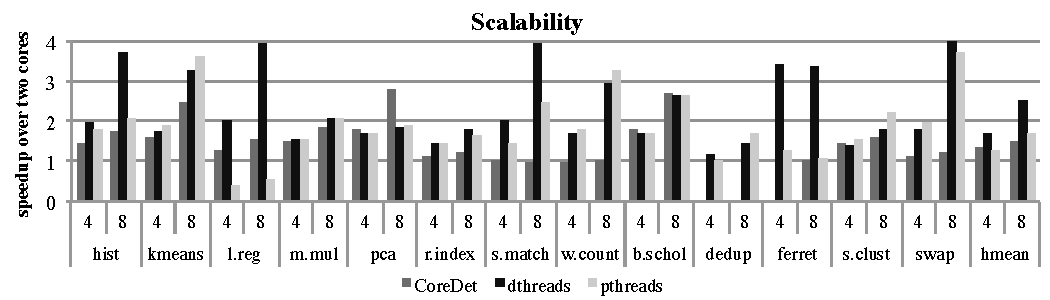
\includegraphics[width=6in]{dthreads/figure/scalability-figure}
\caption{Speedup of eight cores versus two cores (higher is better).  When possible to control with command line options, the number of threads was matched to the number of cores enabled.\label{fig:scalability}}
}
\end{figure}

To measure the scalability cost of running \dthreads{}, we ran two benchmark suite (excluding \texttt{canneal}) on the same machine with eight cores, four cores, and just two cores enabled.  Whenever possible without source code modifications, the number of threads was matched to the number of CPUs enabled.  We have found that \dthreads{} scales at least as well as \pthreads{} for 9 of 13 benchmarks, and scales as well or better than CoreDet for all but one benchmark. On average, \dthreads{} outperforms CoreDet by $3.5\times$.  Detailed results of this experiment are presented in Figure~\ref{fig:scalability} and discussed as follows.

\texttt{canneal} was excluded from the scalability experiment because this benchmark does more work when more threads are present, making the performance comparison between eight and two threads unfair.  \dthreads{} hurts scalability (relative to \pthreads{}) for four of the benchmarks: \texttt{kmeans}, \texttt{word\_count}, \texttt{dedup}, and \texttt{streamcluster}, although only marginally in most cases.  In all of these cases, \dthreads{} scales better than CoreDet.

\dthreads{} is able to match the scalability of \pthreads{} for three benchmarks: \texttt{matrix\_multiply}, \texttt{pca}, and \texttt{blackscholes}.  With \dthreads{}, scalability actually improves over \pthreads{} for 6 out of 13 benchmarks: \texttt{histogram}, \texttt{linear\_regression}, \texttt{reverse\_index}, \texttt{string\_match}, \texttt{ferret}, and \texttt{swaptions}.




\subsection{Performance Analysis}

\subsubsection{Benchmark Characteristics}

The data presented in Table~\ref{tbl:characteristics} are obtained from the executions running on all 8 cores.  Column 2 shows the percentage of time spent in serial phases.  In \dthreads{}, all memory commits and actual synchronization operations are performed in serial phases.  The percentage of time spent in serial phases thus can affect performance and scalability. Applications with higher overhead in \dthreads{} often spend a higher percentage of time in
serial phases, primarily because they modify a large number of pages that need to be committed during serial phases.

Column 3 shows the number of transactions in each application and Column 4 provides the average length of each transaction (ms).  Every synchronization, including locks, conditional variable, barriers, and thread exits, demarcate transaction boundaries in \dthreads{}.  For example, \texttt{reverse\_index}, \texttt{dedup}, \texttt{ferret}
and \texttt{streamcluster} perform numerous transactions whose
execution time is less than 1ms, imposing a performance penalty for these applications.  Benchmarks with longer (or fewer) transactions run almost the same speed as or faster than \texttt{pthreads}, including \texttt{histogram} or \texttt{pca}.  In \dthreads{}, longer transactions amortize the overhead of memory protection and copying over a longer period, thus reducing performance overhead.

Column 5 and 6 provides more detail on the costs associated with memory updates (the number and total volume of dirtied pages). From the table, it is clear why \texttt{canneal} (the most notable outlier) runs much slower with \dthreads{} than with \pthreads{}. This benchmark updates over three million pages, leading to large performance overhead caused by creating private copies, handling protection faults, and committing modifications on those pages to the shared memory mapping. 

\textbf{Conclusion: }
Most benchmarks examined here contain either a small number of transactions, thus having long running transactions, and modify a modest number of pages during execution. For these applications, \dthreads{} is able to amortize its overhead: by eliminating false sharing, it can even run faster than \pthreads{}. However, for the few benchmarks that perform numerous short-lived transactions, or modify a large amount of pages, \dthreads{} can introduce substantial overhead.


\begin{table*}[!t]
\centering
\resizebox{\columnwidth}{!}{
\begin{tabular}{l|rrrrr}
& {\bf \small Serial Phase} & {\bf \small Transactions} & {\bf \small TransLength} & {\bf \small DirtyPages} & {\bf \small DirtyPages}
\\
{\bf \small Benchmark} & {\bf \small (\% of time)} & {\bf (\#)} & {\bf \small (ms)} & {\bf \small (\#)} & {\bf \small (GB)}\\
%\hline
%\multicolumn{6}{|c|}{\emph{Phoenix}} \\
\hline
\small \textbf{histogram} & 0 & 23 & 15.47 & 29 & 0 \\
\small \textbf{kmeans} & 0 & 3929 & 3.82 & 9466 & 0.04\\
\small \textbf{linear\_regression} & 0 & 24 & 23.92 & 17 & 0\\
\small \textbf{matrix\_multiply} & 0 & 24 & 841.2 & 3945 & 0.02\\
\small \textbf{pca} & 0 & 48 & 443 & 11471 & 0.04 \\
\small \textbf{reverseindex} & 17\% & 61009 & 1.04 & 451876 & 1.72\\
\small \textbf{string\_match} & 0 & 24 & 82 & 41 & 0 \\
\small \textbf{word\_count} & 1\% & 90 & 26.5 & 5261 & 0.02\\
%\hline
%\multicolumn{6}{|c|}{\emph{PARSEC}} \\
%\hline
\small \textbf{blackscholes} & 0 & 24 & 386.9 & 991 & 0\\
\small \textbf{canneal} & 26.4\% & 1062 & 43 & 3606413 & 13.75\\
\small \textbf{dedup} & 31\% & 45689 & 0.1 & 356589 & 1.36\\
\small \textbf{ferret} & 12.3\% & 484127 & 0.05 & 844184 & 3.21 \\
\small \textbf{streamcluster} & 18.4\% & 130001 & 0.04 & 131992 & 0.50\\
\small \textbf{swaptions} & 0 & 24 & 163 & 867 & 0\\
\hline
\end{tabular}
}
\caption{Benchmark characteristics.\label{tbl:characteristics}}
\end{table*}

\subsubsection{Performance Impact Analysis}
We further evaluate the performance impact of two important components of \dthreads: deterministic synchronization (sync-only) and memory protection(prot-only).

\emph{Sync-only}: This configuration enforces a deterministic synchronization order. However, memory protection is not enabled so all ``threads'' (actually processes) access the shared memory directly. We want to use this to show the performance impact of load imbalance, caused by synchronization based scheduling.

\emph{Prot-only}: This configuration runs threads in isolation, and commits at synchronization points. The order of synchronization and memory commits are non-deterministic. This configuration eliminates false sharing, but also introduces the performance overhead of isolation and memory commits. In order to guarantee correct execution, we replaced those synchronizations as corresponding cross-processes synchronizations. The lazy twin creation and single-threaded execution optimizations are disabled here because they are unsafe without deterministic synchronization. Thus, this configuration actually evaluates the performance of the \sheriff{} framework. 


\begin{figure*}[!t]
{\centering
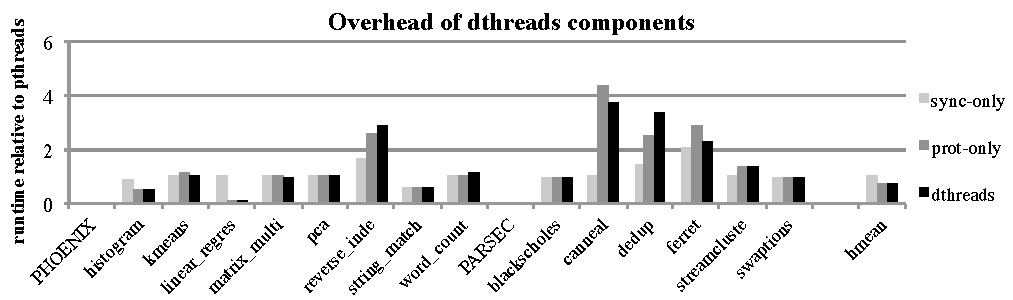
\includegraphics[width=6in]{dthreads/figure/perfeffect}
\caption{Normalized execution time with respect to \pthreads{} (lower is better) for three different configurations. 
\label{fig:perfanalysis}}
}
\end{figure*}

The performance results of these two configurations are shown in Figure~\ref{fig:perfanalysis} and discussed in the following.

\begin{itemize}

\item
The \texttt{reverse\_index}, \texttt{dedup} and \texttt{ferret} benchmarks show significant load imbalance under {\it sync-only} configuration. Additionally, these benchmarks introduces significant overhead with {\it prot-only} configuration because of a large number of transactions there. That explains why \dthreads{} doesn't have good performance on these benchmarks.

\item
The \texttt{string\_match} benchmark shows performance improvement with {\it sync-only} configuration. The exact reason is not clear, may be due to our custom memory allocator (described in Section~\ref{sec:customheap}) that eliminates false sharing problems. 

\item
The \texttt{linear\_regression}, \texttt{histogram} and \texttt{swaptions} benchmarks improve performance with {\it prot-only} configuration. The memory isolation mechanism eliminates false sharing problems inside and contributes to the performance speedup.

\item
Normally the performance of \dthreads{} is not better than the performance of the {\it prot-only} configuration. However, both \texttt{ferret} and \texttt{canneal} run faster with determinism enabled (under \dthreads{}). Both are benefited from specific optimization described in Section~\ref{sec:dthreads-optimization}. \texttt{ferret} benefits from the \emph{single-threaded-execution}. The performance improvement of \texttt{canneal} is coming from the shared twin pages for all threads in parallel phases.

\end{itemize}





